\documentclass[12pt,a4paper]{article}

\usepackage[utf8]{inputenc}
\usepackage[T1]{fontenc}
\usepackage[polish]{babel}
\usepackage{lmodern}
\usepackage{geometry}
\usepackage{graphicx}
\usepackage{array}
\usepackage{longtable}
\usepackage{booktabs}
\usepackage{hyperref}
\usepackage{float}
\usepackage{enumitem}

\geometry{margin=2.5cm}
\setlength{\parindent}{0pt}
\setlength{\parskip}{0.6em}
\hypersetup{colorlinks=true, linkcolor=black, urlcolor=blue}

\newcommand{\frontpage}{%
\begin{titlepage}
    \thispagestyle{empty}
    \begin{minipage}[t]{0.73\textwidth}
        \centering
        \begin{tabular}{|p{0.28\textwidth}|p{0.38\textwidth}|}
            \hline
            \multicolumn{2}{|c|}{\large Struktury danych} \\
            \hline
            \textbf{Kierunek} & \textbf{Termin} \\
            Informatyczne Systemy Automatyki & środa TP 15$^{15}$ -- 16$^{55}$ \\
            \textbf{Imię, nazwisko, numer albumu} & \textbf{Data} \\
            Paweł Bijak 284109, Igor Olewicz 284126 & 8.06.2026 \\
            \textbf{Link do projektu} & \textbf{Temat} \\
            \url{https://github.com/bijakpawel/projekt_SD_sortowanie} & Miniprojekt 3 -- tablica mieszająca \\
            \hline
        \end{tabular}
    \end{minipage}
    \hfill
    \begin{minipage}[t]{0.22\textwidth}
        \centering
        \vspace{0.7cm}
        \IfFileExists{politechnika.png}{%
            \includegraphics[width=0.7\textwidth]{politechnika.png}%
        }{%
            \fbox{\parbox[c][3.2cm][c]{2.2cm}{\centering Politechnika\\Wrocławska}}%
        }
    \end{minipage}

    \vspace{1.6cm}

    {\centering\Large SPRAWOZDANIE -- MINIPROJEKT NR 3\par}
    \vspace{0.4cm}
    \hrule
    \vspace{1.6cm}
\end{titlepage}
}

\begin{document}
\frontpage

\tableofcontents
\newpage

\section{Wstęp teoretyczny}

Tablica mieszająca (ang. \textit{hash table}) jest strukturą danych przeznaczoną do szybkiego przechowywania i wyszukiwania par klucz--wartość. Podstawą działania jest funkcja mieszająca, która odwzorowuje klucz na indeks w tablicy kubków. Jakość tej funkcji oraz sposób obsługi kolizji bezpośrednio wpływają na wydajność całej struktury.

W ramach projektu zaimplementowano trzy warianty tablicy mieszającej:
\begin{itemize}[leftmargin=1.5em]
    \item tablicę z łańcuchowaniem kolizji, gdzie każdy kubełek jest listą rekordów,
    \item tablicę z adresowaniem otwartym i liniowym sondowaniem,
    \item tablicę, w której każdy kubełek stanowi zbalansowane drzewo AVL.
\end{itemize}

W praktyce takie podejścia różnią się nie tylko sposobem rozwiązywania kolizji, ale również zachowaniem przy zwiększaniu liczby elementów. Łańcuchowanie zapewnia prostą implementację i stabilne własności przy umiarkowanym zapełnieniu. Adresowanie otwarte korzysta z jednego ciągłego bufora, co zwykle daje bardzo dobre własności pamięci podręcznej, ale wymaga ostrożnego kontrolowania współczynnika zapełnienia. Z kolei kubełki AVL oferują uporządkowaną strukturę wewnętrzną, dzięki czemu operacje wewnątrz pojedynczego kubełka zachowują logarytmiczną złożoność względem liczby elementów w tym kubełku.

\section{Badania wydajnościowe}

Pomiary przeprowadzono dla trzech implementacji: \texttt{ChainingHashTable}, \texttt{LinearProbingHashTable} oraz \texttt{AvlBucketHashTable}. Dla każdego rozmiaru zbioru generowano losowe pary klucz--wartość, a następnie mierzono średni czas wykonania dwóch operacji:
\begin{itemize}[leftmargin=1.5em]
    \item \texttt{insert} -- wstawienie nowej pary do słownika,
    \item \texttt{remove} -- usunięcie pary powiązanej z kluczem.
\end{itemize}

Czasy zapisano w nanosekundach, a pomiary wykonano dla rozmiarów od 5000 do 100000 elementów. Wyniki zestawiono na wykresach porównawczych na rysunkach \ref{fig:insert} i \ref{fig:remove}.

\begin{figure}[H]
    \centering
    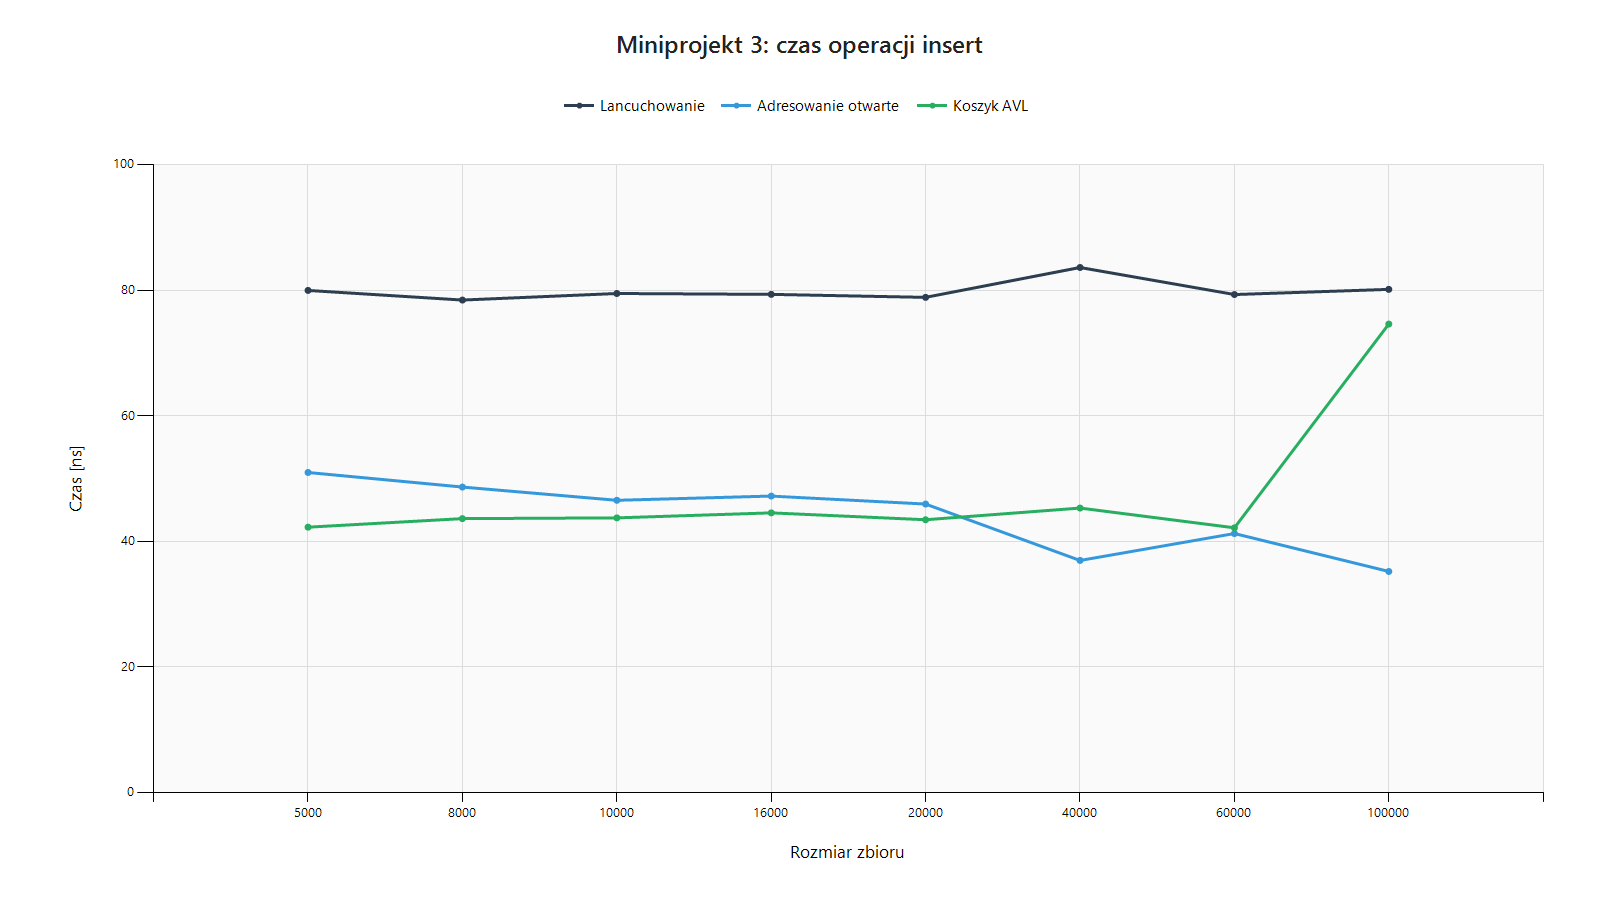
\includegraphics[width=0.92\textwidth]{wykresy/wykres_insert_final.png}
    \caption{Porównanie czasu operacji insert}
    \label{fig:insert}
\end{figure}

\begin{figure}[H]
    \centering
    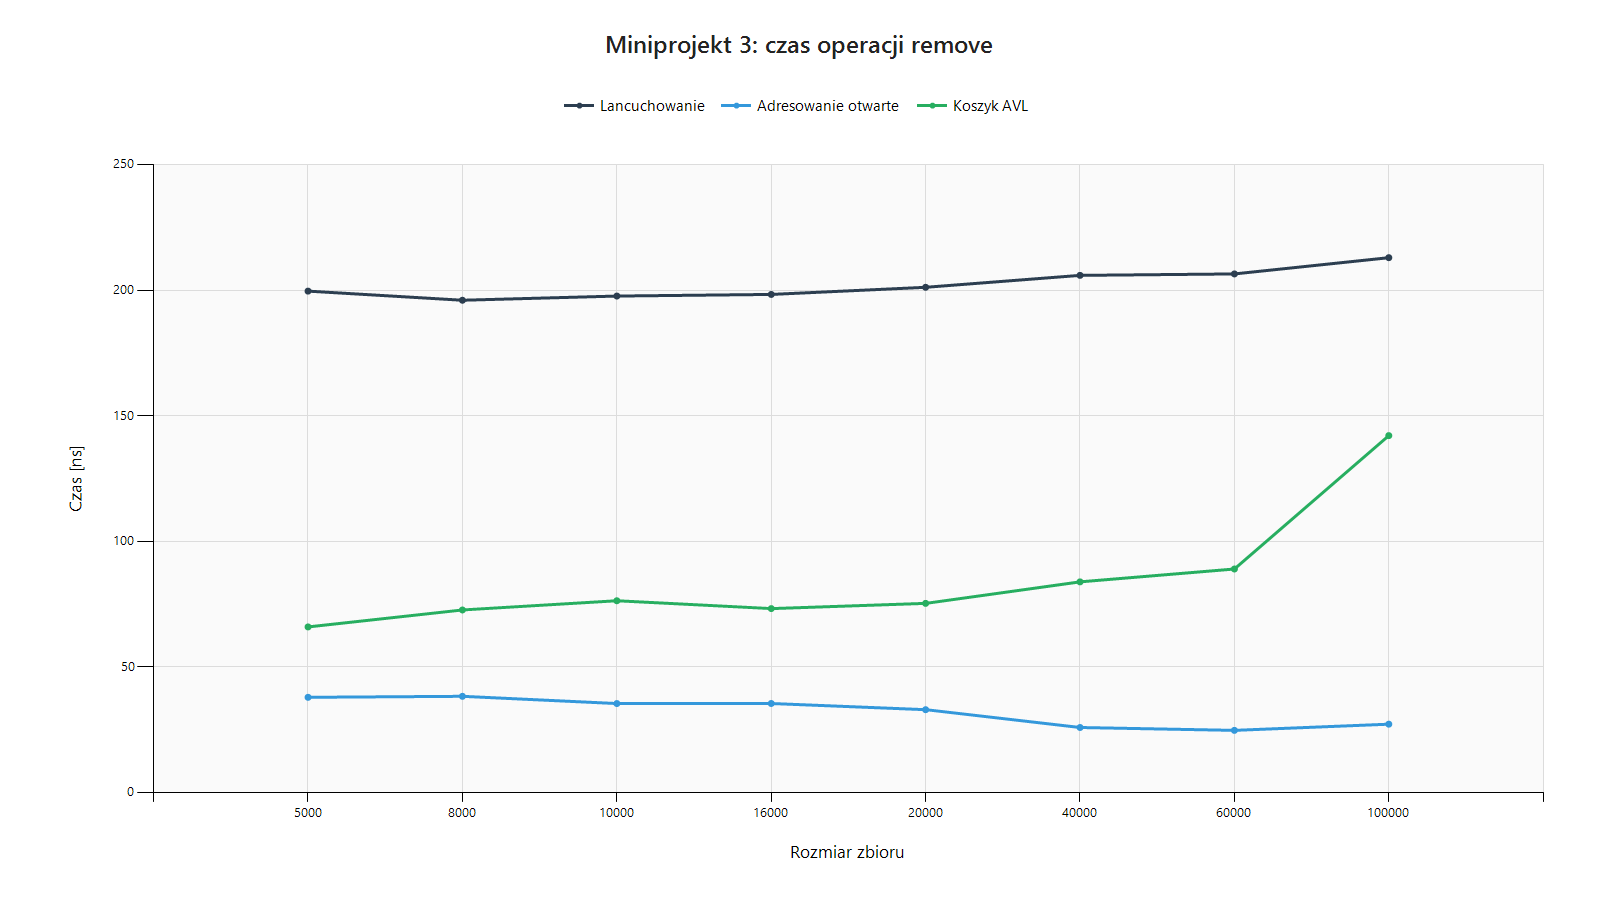
\includegraphics[width=0.92\textwidth]{wykresy/wykres_remove_final.png}
    \caption{Porównanie czasu operacji remove}
    \label{fig:remove}
\end{figure}

\subsection*{Opis wyników}

Dla operacji \texttt{insert} najszybsza okazała się tablica z adresowaniem otwartym. Jej czasy pozostawały najniższe w całym zakresie testowanych rozmiarów i zwykle mieściły się w przedziale około 35--51 ns. Tablica z łańcuchowaniem była wolniejsza, ale nadal stabilna -- najczęściej około 78--84 ns. Największe czasy uzyskał wariant z kubełkami AVL, gdzie wyniki wynosiły w przybliżeniu 42--75 ns, z wyraźnym wzrostem dla największego zbioru.

W przypadku operacji \texttt{remove} najlepsze wyniki ponownie dało adresowanie otwarte, z czasami około 24--38 ns. Łańcuchowanie było znacznie wolniejsze i utrzymywało się głównie w okolicach 196--213 ns. Wariant z kubełkami AVL zajmował pozycję pośrednią, ale przy największym rozmiarze danych widoczny jest silny wzrost kosztu usuwania do około 142 ns.

\begin{table}[H]
\centering
\caption{Średnie czasy wykonania operacji insert [ns]}
\begin{tabular}{rccc}
\toprule
Rozmiar & Łańcuchowanie & Adresowanie otwarte & Koszyk AVL \\
\midrule
5000 & 79,9703 & 50,9813 & 42,2795 \\
10000 & 78,4364 & 48,6675 & 43,6439 \\
15000 & 79,4833 & 46,5514 & 43,7595 \\
16000 & 79,3423 & 47,2273 & 44,5573 \\
20000 & 78,8686 & 45,9556 & 43,4567 \\
40000 & 83,6242 & 36,9798 & 45,3241 \\
60000 & 79,3192 & 41,2648 & 42,1781 \\
100000 & 80,1366 & 35,2258 & 74,6192 \\
\bottomrule
\end{tabular}
\end{table}

\begin{table}[H]
\centering
\caption{Średnie czasy wykonania operacji remove [ns]}
\begin{tabular}{rccc}
\toprule
Rozmiar & Łańcuchowanie & Adresowanie otwarte & Koszyk AVL \\
\midrule
5000 & 199,6550 & 37,9759 & 65,9872 \\
10000 & 196,0210 & 38,3759 & 72,7397 \\
15000 & 197,6910 & 35,4958 & 76,4028 \\
16000 & 198,3360 & 35,5177 & 73,2870 \\
20000 & 201,1740 & 33,0573 & 75,3553 \\
40000 & 205,9230 & 25,9556 & 83,9211 \\
60000 & 206,4980 & 24,8205 & 89,0497 \\
100000 & 212,9560 & 27,2677 & 142,1350 \\
\bottomrule
\end{tabular}
\end{table}

\section{Wnioski}

Przeprowadzone pomiary pokazują, że wybór wariantu tablicy mieszającej powinien zależeć od dominujących operacji oraz oczekiwanego obciążenia struktury.

\subsection{Wstawianie elementów}
Najlepsze wyniki dla operacji \texttt{insert} uzyskało adresowanie otwarte. Wynika to z prostego modelu przechowywania danych w jednym buforze oraz z bardzo dobrych własności lokalności pamięci. Łańcuchowanie jest stabilne, ale przeciętnie wolniejsze. Kubełki AVL zapewniają porządek wewnątrz kubełka, lecz koszt utrzymania drzewa równoważonego jest widoczny przy większej liczbie elementów.

\subsection{Usuwanie elementów}
W przypadku \texttt{remove} adresowanie otwarte ponownie wypada najlepiej. Łańcuchowanie ma znacznie wyższy i bardziej płaski koszt, co sugeruje większy narzut związany z przeszukiwaniem kubełka listowego. Wariant AVL jest kompromisem pomiędzy prostotą łańcuchowania a uporządkowaniem danych, ale przy dużych zbiorach może wyraźnie tracić wydajność.

\subsection{Ocena ogólna}
Jeżeli priorytetem są możliwie najkrótsze czasy pojedynczych operacji, najlepszym wyborem w badanym zestawie okazało się adresowanie otwarte. Łańcuchowanie pozostaje rozwiązaniem prostym i przewidywalnym, natomiast kubełki AVL są najciekawsze tam, gdzie oprócz samego rozwiązywania kolizji zależy nam na uporządkowanej strukturze w obrębie kubełka.

\end{document}
